\section{Livello 1: Physic}
    \subsection{Scopo e caratteristiche del livello}
        Il \textit{livello fisico} si occupa del trasferimento fisico dei bit sul canale di comuni- cazione che interconnette due o più nodi adiacenti.

        Il trasferimento avviene utilizzando un mezzo trasmissivo su cui i bit vengono codificati, trasformandoli in una forma di energia (tipicamente, segnali elettromagnetici come: luce, tensione, onde elettromagnetiche).

        I nodi sono dotati di un adattatore, che ha il compito di codificare i bit in uscita e decodificare i bit in arrivo.

        Nelle reti di comunicazione, esistono due tipologie principali di canali ad acesso diretto:
        \begin{itemize}
            \item Punto-punto (1-1)
            \item Multi-accesso (1-N)
            \begin{itemize}
                \item Broadcast (1-Tutti)
                \item Multicast (1-N)
            \end{itemize}
        \end{itemize}

        Esistono tre categorie principali di mezzi fisici per la realizzazione di un canale:
        \begin{itemize}
            \item Elettrico: cavi coassiali di rame (multi-accesso) e doppini telefonici (punto-punto).
            \item Ottico: fibre ottiche (Punto-Punto).
            \item Wireless: onde radio omnidirezionali (multi-accesso); ponti radio (punto-punto); satelliti (punto-punto o multi-accesso).
        \end{itemize}

    \subsection{Caratteristiche fisiche del segnale}
        \subsubsection{Attenuazione}
            L'\textit{attenuazione} è la diminuzione del segnale sulla lunghezza del mezzo. Determina la massima lunghezza utilizzabile, è dovuto ad una perdita di energia.

            Dati P$_1$ = trasmittente, e P$_2$ = ricevente

            \begin{equation*}
                attenuazione = 10 \cdot log_{10} \left( \frac{P2}{P1}\right) ~ [db]
            \end{equation*}

            Un dimezzamento di potenza nel segnale equivale a:
            \begin{math}
                10 \cdot log_{10} \left( \frac{P_2}{P_1}\right) = -3db
            \end{math}

            Un raddoppio della potenza del segnale equivale a:
            \begin{math}
                10 \cdot log_{10} \left( \frac{P_2}{P_1}\right) = 3db
            \end{math}

        \subsubsection{Banda Passante [H]}
            La \textit{banda passante} è l'attenuazione in funzione della frequenza, è il range di frequenze trasportate dal mezzo trasmissivo.
        
            Viene determinata dalle caratteristiche fisiche del mezzo.

        \subsubsection{Distorsione}
            Se le frequenze che compongono il segnale subiscono attenuazioni diverse, si ha una distorsione del segnale.

        \subsubsection{Rumore}
            Al segnale con potenza $S$, si sovrappone il rumore termico con potenza $N$, sempre presente dovuto al movimento delle molecole del mezzo.
        
            Il rapporto \textbf{Signal Noise Ratio (SNR)} si misura in decibel:
            \begin{math}
                10 \cdot log_{10} \left( \frac{S}{N}\right)
            \end{math}1
        
        \subsubsection{Disturbo}
            Proveniente da elementi esterni, ad esempio da canali adiacenti.

        \subsubsection{Teorema di Nysquit}
            Il \textit{teorema di Nysquit} spiega la relazione tra la banda passante ed il bitrate su un canale ideale privo di rumore.

            Sia $H$ la banda passante, e $V$ il numero di livelli discreti del segnale:

            \begin{equation*}
                bitrate = 2H \cdot log_2(V) ~ [bit/s]
            \end{equation*}

            Da cui segue che:

            \begin{equation*}
                V = 2^{\frac{bitrate}{2H}}
            \end{equation*}

        \subsubsection{Teorema di Shannon}
            Il \textit{teorema di Shannon} spiega la relazione tra la banda passante, il bitrate ed il rapporto SNR.

            \begin{equation*}
                bitrate = H \cdot log_2(1 + SNR) ~ [bit/s]
            \end{equation*}

        \subsubsection{Tempo di propagazione}
            Il \textit{tempo di propagazione} è il tempo che impiega un bit a percorre il mezzo trasmissivo.

            Siano $I$ la lunghezza del mezzo, $v$ la velocità di propagazione del mezzo: 
            \begin{math}
                v_{aria} = 3 \cdot 10^8 ~ m/s; ~ v_{fibra/rame} = 2 \cdot 10^8 ~ m/s
            \end{math}

            \begin{equation*}
                t_{pr} = \frac{I}{v} ~ [s]
            \end{equation*}

        \subsubsection{Tempo di trasmissione}
            Il \textit{tempo di trasmissione} è il tempo che impiega una sequenza di bit ad uscire dall'interfaccia di rete.

            \begin{equation*}
                t_{tr} = \frac{\#bit}{bitrate} ~ [s]
            \end{equation*}

        \subsubsection{Tempo di elaborazione}
            Il \textit{tempo di elaborazione} ($t_{elab}$) è il tempo dovuto al processamento dei dati e dipende dalle caratteristiche hardware dei nodi in transito.
            
        \subsubsection{Tempo di attesa}
            Il \textit{tempo di attesa} è il tempo relativo alle attese nelle code di trasmissione. Dipende dal carico della rete, ed è trascurabile se la rete è scarica.

        \subsubsection{Tempo di riempimento del pacchetto}
            Se abbiamo un flusso continuo di dati, i primi bit inseriti in un pacchetto devono attendere il completamento del pacchetto prima di essere inviati.

        \subsubsection{Round Time Trip (RTT)}
            L'RTT è il tempo di andata e ritorno di un bit.

            \begin{equation*}
                RTT = 2 \cdot t_{pr}
            \end{equation*}

    \subsection{Mezzi fisici di propagazione}
        \subsubsection{Cavo coassiale}
            È comptituito da due cavi di rame concentrici e serve per tramissioni multi-accesso e/o half-duplex.

            Veniva utilizzato negli anni '80-'90 per reti locali, attualmente diffuso per la TV via cavo.

        \subsubsection{Doppino}
            È una coppia di fili di rame avvolti non schermati. Permettono una banda passante fino a 600 Mhz, cioè fino a un massimo di 10 Gb/s, l'attenuazione consente trasmissione fino a un massimo di 100-200 metri.

        \subsubsection{Fibra ottica}
            Sono fibre di vetro che trasportano impulsi di luce su fibre flessibili del diametro di qualche decina di $\mu m$.
        
            Hanno tre componenti: la sorgente luminosa, il mezzo di trasmissione ed il rilevatore.
        
            Possono avere una modulazione in cui un impulso di luce indica il valore 1, mentre l'assenza indica il valore 0, oppure possono modulare una portante.

            Hanno un ottimo rapporto SNR (60$\sim$65 dB), ed un elevata capacità trasmissiva (fino a 50 $Tbps$), una bassa attenuazione ed è immune da disturbi elettromagnetici; è sicura (difficoltà di inserimento nella comunicazione), minor dimensione e maggiore costo di installazione rispetto all'alternativa in rame.

            Esistono due tipi di fibre ottiche:
            \begin{itemize}
                \item \textbf{Fibre multimodali}: i raggi colpiscono le pareti con diverse angolazioni, vengono utilizzate per brevi distanze, la luce viene genarata tramite LED.
                \item \textbf{Fibre monomodali}: i raggi vengono spediti in un percorso rettilineo, senza rimbalzi, vengno utilizzate per le lunghe distanze, hanno maggiore costo ma minore attenuazione.
            \end{itemize}

    \subsection{Onde elettromagnetiche}
        Le onde elettromagnetiche possono essere utilizzate per trasmettere informazioni senza l'utilizzo di un mezzo fisico guidato.

        La trasmissione dei dati avviene modulando l'\textbf{ampiezza}, la \textbf{frequenza} o la \textbf{fase} dell'onda.

        Le onde vengono misurate in base alla loro frequenza (f) [Hz] o lunghezza $\lambda$ [m].

        Le due grandezze sono legate dalla velocità della luce nel vuoto (c):

        \begin{equation*}
            c = \lambda f
        \end{equation*}

    \subsection{Spettro elettromagnetico}
        \subsubsection{Onde radio ($10^4\sim10^9 ~[Hz]$)}
            Sono facili da generare, possono viaggiare per lunghe distanze ed attraversano i corpi solidi. Il loro limite è dato dalla ridotta ampiezza di banda.
            
            Le onde radio (LF, MF e HF) seguono il terreno; mentre le VHF e UHF viaggiano in linea retta e rimbalzano contro gli ostacoli.

        \subsubsection{Microonde ($10^9\sim10^{11} ~[Hz] - \frac{\lambda}{10}[cm]$)}
            Viaggiano in linea retta e faticano ad attraversare corpi solidi, sono adatte per connessioni punto-punto (con visibilità ottica).

        \subsubsection{Infrarossi ($10^{11}\sim4 \cdot 10^{14} ~[Hz] - \frac{\lambda}{1}[\mu m]$)}
            Non attraversano gli ostacoli solidi, sono utilizzati per periferiche a breve distanza (telecomandi) e per gli impulsi nelle fibre ottiche.

        \subsubsection{Luce visibile ($4 \cdot 10^{14}\sim8 \cdot 10^{14} ~[Hz] - \frac{\lambda}{0.5}[\mu m]$)}
        
        \subsubsection{Luce ultravioletta, raggi x, raggi gamma ($>8 \cdot 10^{14} ~[Hz]$)}
            Sono difficili da generare, da modulare, non si propagano bene attraverso i corpi solidi e sono dannose.

        \subsubsection{Utilizzo dello spettro}
            Al crescere della frequenza aumenta l'ampiezza del canale, ma peggiora l'interazione con l'ambiente.

            A tutte le frequenze le onde sono soggette a disturbi (motori ed altri dispositivi elettrici) e ad interferenze con altre trasmissioni dati via etere. Per questo motivo i governi regolano e limitano l'utilizzo delle trasmissioni via radio mediante opportune licenze.

            Molti governi hanno mantenuto libere alcune bande di frequenza, note come bande \textbf{ISM (Industriale Scientifica Medica)}, che possono essere utilizzate da chiunque, senza licenza, a patto di rispettare limiti di potenza per limitarne le interferenze.

            I principali utilizzi per la trasmissione dati sono:
            \begin{itemize}
                \item \textbf{Ponti radio}: connessioni punto-punto terrestri o satellitari, utilizzano per le trasmissioni dati frequenze nel campo dei GHz, e quindi lunghezze d'onda dell'ordine del centimetro, per cui le antenne impiegate sono necessariemente del tipo parabolico.
                \item \textbf{Reti locali}: connessioni omnidirezionali utilizzate all'interno degli edifici per realizzare reti multiaccesso. Si utilizzano microonde per minimizzare i problemi di attraversamento delle pareti. L'ampiezza può arrivare fino a 50 Mb/s in un raggio di 100 - 200 metri (WiFi) o qualche chilometro (WiMax).
            \end{itemize}

    \subsection{Codifiche dei bit}
        Il trasferimento dei bit avviene codificando sul canale due o più simboli, il numero dei simboli trasmessi in un secondo è detto \textbf{baud-rate}.

        Le principali tecniche di codifica sono:
        \begin{itemize}
            \item Codifica di linea: trasmissione in banda base
            \item Trasmissione in banda passante:
                \begin{itemize}
                    \item Modulazione di una frequenza portante
                    \item Diffusione dello spettro
                \end{itemize}
        \end{itemize}

        \subsubsection{Codifica di linea}
            La codifica di linea è il processo di conversione di dati digitali in segnali digitali (livelli o transizioni di tensione).
        
            La comunicazione è generalmente seriale: si utilizza un solo canale. I simboli vengono codificati all'interno di intervalli di tempo costante (\textbf{clock}) che rappresentano il sincronismo condiviso tra trasmettitore e ricevitore.

            \subsubsection*{Modalità asincrona}
            Ogni gruppo di bit è inviato in modo asincrono; ogni gruppo è preceduto da una sequenza di bit aggiuntivi che consentono al destinatario di ricostruire il sincronismo. Questa è la modalità utilizzata nelle reti calcolatori.

            \subsubsection*{Modalità sincrona}
            Non sono previsti bit di sincronismo. Il segnale di clock viene inviato parallelamente al canale dei dati, oppure il flusso non viene mai interrotto per non perdere il sincronismo. Generalmente questo è possibile solo per connessioni a breve distanza ed alta velocità.

        \subsubsection{Schemi di codifica di linea: RZ e NRZ}
            \begin{center}
    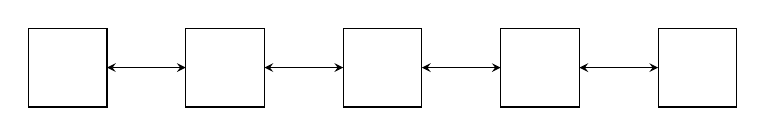
\begin{tikzpicture}
        %%%%%%%%%% Nodi %%%%%%%%%%
        \foreach \x in {0,2,...,8}
            \draw (\x,0) rectangle ++(1,1);

        %%%%%%%%% Frecce %%%%%%%%%
        \foreach \x in {1,3,...,7}
            \draw[<->,>=stealth] (\x,0.5) -- ++(1,0);
    \end{tikzpicture}
\end{center}

            \subsubsection*{NRZ}
            Non richiede circuiti complicati: i dati sono passati direttamente in uscita, è robusto agli errori ma lunghe stringhe di zeri o uni causano perdita di sincronismo.

            \subsubsection*{RZ}
            e più soggetto ad errori, ma non perde di sincronismo perché lo stato cambia ad ogni bit.

            RZ e NRZ vengono usate nella trasmissione PCM (trasmissione telefonica digitale).

        \subsubsection{Schemi di codifica di linea: NRZ-I e Manchester}
            \begin{center}
    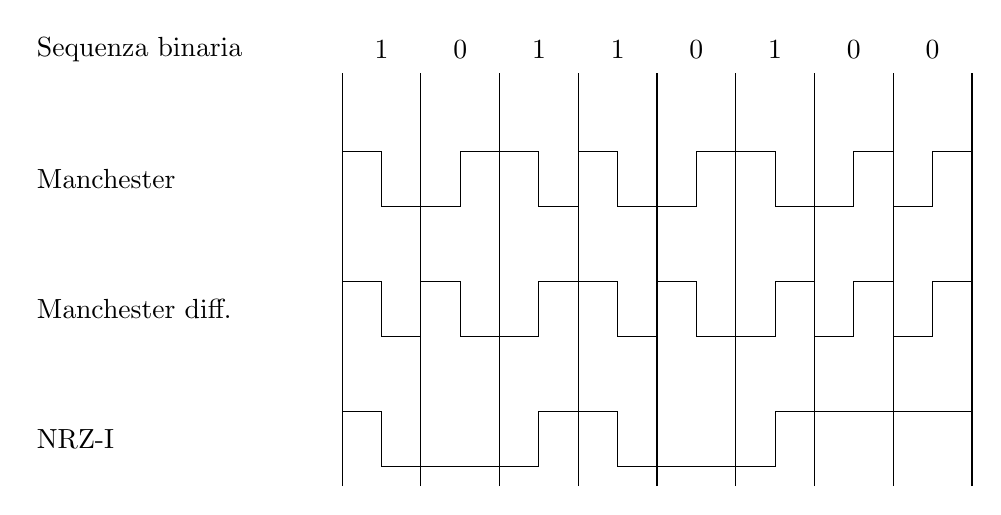
\begin{tikzpicture}
        %%%%%%%%% Barre %%%%%%%%%%
        \foreach \x in {4,...,12}
            \draw (\x,-0.25) -- (\x,5);

        %%%%%%%%% Numeri %%%%%%%%%
        \node at (4.5,5.3) {1};
        \node at (5.5,5.3) {0};
        \node at (6.5,5.3) {1};
        \node at (7.5,5.3) {1};
        \node at (8.5,5.3) {0};
        \node at (9.5,5.3) {1};
        \node at (10.5,5.3) {0};
        \node at (11.5,5.3) {0};

        %%%%%%%%% NRZ-I %%%%%%%%%%
        \draw (4,0.7) -- (4.5,0.7) -- (4.5,0) -- (6.5,0) -- (6.5,0.7) -- (7.5,0.7) -- (7.5,0) -- (9.5,0) -- (9.5,0.7) -- (12,0.7);

        %%%% Manchester Diff. %%%%
        \draw (4,2.35) -- (4.5,2.35) -- (4.5,1.65) -- (5,1.65);
        \draw (5,2.35) -- (5.5,2.35) -- (5.5,1.65) -- (6,1.65);
        \draw (6,1.65) -- (6.5,1.65) -- (6.5,2.35) -- (7,2.35);
        \draw (7,2.35) -- (7.5,2.35) -- (7.5,1.65) -- (8,1.65);
        \draw (8,2.35) -- (8.5,2.35) -- (8.5,1.65) -- (9,1.65);
        \draw (9,1.65) -- (9.5,1.65) -- (9.5,2.35) -- (10,2.35);
        \draw (10,1.65) -- (10.5,1.65) -- (10.5,2.35) -- (11,2.35);
        \draw (11,1.65) -- (11.5,1.65) -- (11.5,2.35) -- (12,2.35);

        %%%%%%% Manchester %%%%%%%
        \draw (4,4) -- (4.5,4) -- (4.5,3.3) -- (5,3.3);
        \draw (5,3.3) -- (5.5,3.3) -- (5.5,4) -- (6,4);
        \draw (6,4) -- (6.5,4) -- (6.5,3.3) -- (7,3.3);
        \draw (7,4) -- (7.5,4) -- (7.5,3.3) -- (8,3.3);
        \draw (8,3.3) -- (8.5,3.3) -- (8.5,4) -- (9,4);
        \draw (9,4) -- (9.5,4) -- (9.5,3.3) -- (10,3.3);
        \draw (10,3.3) -- (10.5,3.3) -- (10.5,4) -- (11,4);
        \draw (11,3.3) -- (11.5,3.3) -- (11.5,4) -- (12,4);

        %%%%%%%% Legenda %%%%%%%%%
        \node[anchor=west] at (0,5.3) {Sequenza binaria};
        \node[anchor=west] at (0,3.65) {Manchester};
        \node[anchor=west] at (0,2) {Manchester diff.};
        \node[anchor=west] at (0,0.35) {NRZ-I};
    \end{tikzpicture}
\end{center}

            \textbf{NRZ-I} cambia il simbolo di codifica in corrispondenza del bit 1, altrimenti rimane invariato.

            La codifica \textbf{Manchester}, codificando i bit con le transizioni, è invece ideale per la gestione del sincronismo e per questo è utilizzata nel protocollo \textbf{Ethernet 10baseT}. Da notare che la codifica Manchester invia segnali ad una frequenza doppia.

            La codifica \textbf{Manchester differenziale} combina la codifica Manchester con quella NRZ-I.

        \subsubsection{Codifiche a blocchi}
            La codifica a blocchi viene solitamente chiamata \textbf{mB/nB}: trasforma una parola sorgente di $m$ bit in una parola codice di $n$ bit ($n > m$). Introduce una maggiore ridondanza per diminuire il tasso di errori.
        
            La codifica a blocchi \textbf{4B5B} viene utilizzata per \textbf{FastEthernet}: sequenze di 4 bit sono codificate in sequenze di 5 bit, con un bit aggiuntivo che ha il compito di garantire almeno una transizione per blocco.

            Le sequenze generate vengono inviate con la codifica NRZ-I:
            \begin{itemize}
                \item Occorre una larghezza di banda maggiorata del 25\%
                \item È utilizzata da 100baseTX con 125 Baud/s, ovvero 100 bps.
            \end{itemize}

        \subsubsection{Modulazione di una frequenza portante}
            La codifica delle onde elettromagnetiche avviene modulando l'ampiezza, la frequenza o la fase (o una combinazione di questi metodi) di un'onda portante.

            \begin{center}
    \begin{tikzpicture}
        %%%%%%%%%% Nodi %%%%%%%%%%
        \draw (0.8,0) rectangle (1.8,1);
        \draw (3.2,0) rectangle (4.2,1);
        \draw (0,2.2) rectangle (1,3.2);
        \draw (4,2.2) rectangle (5,3.2);
        \draw (2,4) rectangle (3,5);
        \draw (2,1.8) rectangle (3,2.8);

        %%%%%%%%% Frecce %%%%%%%%%
        \draw[<->,>=stealth] (1.3,1) -- (2,1.8);
        \draw[<->,>=stealth] (3.7,1) -- (3,1.8);
        \draw[<->,>=stealth] (1,2.8) -- (2,2.6);
        \draw[<->,>=stealth] (3,2.6) -- (4,2.8);
        \draw[<->,>=stealth] (2.5,4) -- (2.5,2.8);
    \end{tikzpicture}
\end{center}

        \subsubsection{Diagrammi a costellazione}
            La modulazione combinata di ampiezza e fase è detta \textbf{QAM (Quadrature Amplitude Modulation)}, è la più efficiente ed usata.

            Ogni simbolo è determinato da una coppia ampiezza-fase, rappresentato da un punto del diagramma delle fasi, l'insieme dei punti formano una costellazione.

            \begin{enumerate}[label=(\alph*)]
                \item QPSK: modulazione di fase a quattro stati (2 bit per baud)
                \item QAM16: modulazione di ampiezza e fase a 16 stati (4 bit per baud)
                \item QAM64: modulazione di ampiezza e fase a 64 stati (6 bit per baud)
            \end{enumerate}

            \begin{center}
    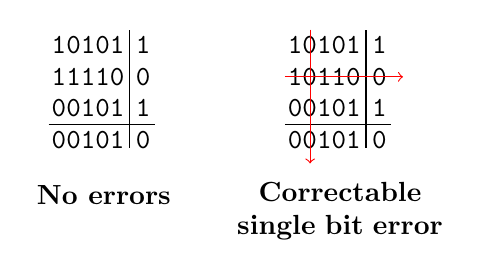
\begin{tikzpicture}
        %%%%%%%% Testo 1 %%%%%%%%%
        \node at (0,0) {\texttt{00101}};
        \node at (0,0.4) {\texttt{00101}};
        \node at (0,0.8) {\texttt{11110}};
        \node at (0,1.2) {\texttt{10101}};
        \node at (0.7,0) {\texttt{0}};
        \node at (0.7,0.4) {\texttt{1}};
        \node at (0.7,0.8) {\texttt{0}};
        \node at (0.7,1.2) {\texttt{1}};

        %%%%%%%% Schema 1 %%%%%%%%
        \draw (0.53,-0.1) -- (0.53,1.4);
        \draw (-0.5,0.2) -- (0.85,0.2);

        %%%%%%%% Testo 2 %%%%%%%%%
        \node at (3,0) {\texttt{00101}};
        \node at (3,0.4) {\texttt{00101}};
        \node at (3,0.8) {\texttt{10110}};
        \node at (3,1.2) {\texttt{10101}};
        \node at (3.7,0) {\texttt{0}};
        \node at (3.7,0.4) {\texttt{1}};
        \node at (3.7,0.8) {\texttt{0}};
        \node at (3.7,1.2) {\texttt{1}};

        %%%%%%%% Schema 2 %%%%%%%%
        \draw (3.53,-0.1) -- (3.53,1.4);
        \draw (2.5,0.2) -- (3.85,0.2);
        \draw[->,red] (2.5,0.8) -- (4,0.8);
        \draw[->,red] (2.82,1.4) -- (2.82,-0.3);

        %%%%%%%% Captions %%%%%%%%
        \node at (0.2,-0.7) {\textbf{No errors}};
        \node[text width=2.7cm,align=center] at (3.2,-0.9) {\textbf{Correctable single bit error}};
    \end{tikzpicture}
\end{center}

        \subsubsection{Multiplexing}
            Quando la larghezza di banda del canale trasmissivo è maggiore della larghezza di banda effettivamente necessaria, il canale può essere condiviso da più trasmissioni simultanee.

            Il \textit{multiplexing} è la tecnica che permette la trasmissione simultanea di più segnali in un singolo canale.

            Esistono diverse tecniche per implementare il Multiplexing; le principali sono:
            \begin{itemize}
                \item \textbf{FDM (Frequency Divsion Multiplexing)}: a divisione di frequenza, analogico.
                \item \textbf{TDM (Time Division Multiplexing)}: a divisione di tempo, digitale.
            \end{itemize}

            \begin{center}
                \includegraphics[scale=0.41]{chapters/2/assets/schema_e.png}
            \end{center}

        \subsubsection{Diffusione dello spettro}
            Lo spettro delle frequenze assegnate viene suddiviso in più portanti per evitare interferenze e intercettazioni, o per distribuire la trasmissione in base al profilo dell'attenuazione.

            \textbf{FHSS (Frequency Hopping Spread Spectrum)} utilizza 79 canali e cambia frequenza centinaia di volte al secondo, in questo modo è resistente alle interferenze radio. Usato in 802.11 ed in Bluetooth.

            \textbf{CDMA (Code Divisione Multiple Access)}: il segnale viene processato in un circuito logico XOR insieme ad un segnale impulsivo (codice) codificato a frequenza più alta. Il segnale trasmesso consumerà così una maggiore larghezza di banda, consentendo però la ricezione di segnali deboli. Molti segnali del genere possono occupare lo stesso canale simultaneamente, utilizzando diversi codici.

            La tecnica CDMA denominata \textbf{DSSS (Direct Sequence Spread Spectrum)} è usata per la telefonia mobile e in WiFi 802.11b e 802.11g, mentre la tecnica \textbf{WCDMA} usata nei sistemi cellulari 3G.

        \subsubsection{OFDM}
            \textbf{OFDM (Orthogonal Frequency Divsion Multiplexing)} è una tecnica FDM in cui le frequenze portanti sono tra loro ortogonali: le fasi di portanti adiacenti sono calcolate in modo da non interferire tra loro.

            $N$ portanti adiacienti compongono un canale che viene utilizzato per una singola tramissione in cui i dati vengono inviati in parallelo.

            Le singolo sotto-portanti possono utilizzare codifiche diverse in base al profilo dell'attenuazione.

            Viene utilizzata in ADSL, Wifi 802.11g e 802.11n, WiMAX e nei sistemi cellulari LTE.

    \subsection{Telefonia}
        \subsubsection{Il sistema telefonico}
            L'orecchio è in grado di distinguere frequenze da 20 a 20 KHz, ma la voce umana è contenuta entro 4 Khz (da 300 a 3400 Hz). Per questo il sistema telefonico è basato su canali con ampiezza di 4 KHz. Le frequenze superiori vengono tagliate con opportuni filtri.
        
            Il collegamento tra la casa e la centralina Telecom è detto \textbf{Ultimo Miglio} (o Local Loop) e può essere realizzato con un doppino di categoria 3.
        
            Nelle tratte principali della rete di telefonia un \textit{codec} converte il segnale in forma digitale e lo riconverte in analogico in prossimità della destinazione. Le interconnessioni tra le centrali di commutazione avvengono grazie a multiplexing di più canali con tecniche FDM o TDM.

        \subsubsection{PCM}
            La conversazione digitale è standardizzata con la tecnica del campionamento \textbf{PCM (Pulse Code Modulation)}.

            Un canale analogico di 4 KHz richiede 8000 campionamenti al secondo, ovvero uno ogni 125 $\mu s$.

            Ogni campionamento avviene generalmente su 8 bit di dati (o 7 bit più il bit di parità), ottenendo così un flusso di \textbf{64 Kbit/s} o (56 Kbit/s).

            PCM definisce anche la codifica per la trasmissione, la quale può essere NRZ o RZ.

            La rete telefonica con canali tradizionali da 4 KHz è stata utilizzata a lungo come canale per trasmissione a distanza di dati fino a 56 Kbit/s mediante i modem: i bit venivano codificati con segnali assimilabili alla voce umana.

            Una rete telefonica a TDM gestisce canali digitali da 64Kbit/s che con ISDN vengono portati fino in casa dell'utente. Per poter fornire una maggiore ampiezza di canale senza modificare il cablaggio delle case è stato introdotta la tecnologia \textbf{xDLS}. Sfrutta la banda dei cavi in categoria 3.

            Il segnale domestico non viene filtrato a 4 KHz, ma a 1.1 MHz.

            La banda da 1.1 MHz è utilizzata con tecnica OFDM:
            \begin{itemize}
                \item La banda viene suddivisa in \textbf{256} canali da $\frac{1.1 MHz}{256} = \textbf{4.3 KHz}$
                \item All'interno di ogni canale si usa la modulazione QAM con un rate di 4K baud.
                \item Il numero massimo di bit per baud è 15.
                \item La massima velocità di un canale è $4K \cdot 15 bit = \textbf{60 Kb/s}$
                \item La massima velocità aggregata è quindi $256 \cdot 60Kb/s \approx \textbf{15 Mb/s}$
            \end{itemize}

    \subsection{ADSL}
        L'ADSL (Asymmetric DSL) è un utilizzo specifico di xDLS, pensato per l'home computing, in cui il download è prevalente. Con ADSL abbiamo:
        \begin{itemize}
            \item Canale 0 (0 $\sim$ 4.3 KHz): per la fonia.
            \item Canali 1-5 (4.3 KHz $\sim$ 25 KHz): non utilizzati per evitare interferenze tra fonia e dati.
            \item Canale 6-30 (25 KHz $\sim$ 138 KHz): 24 canali per l'upload dei dati.
            
            Massimo: 24 $\cdot$ 60 Kb/s = 1.4 Mb/s (effettivi 0.5 Mb/s)
            \item Canale 31-255 (138 KHz $\sim$ 1.1 MHz): 224 canali per il download dei dati.
            
            Massimo: 224 $\cdot$ 60 Kb/s = 13.4 Mb/s (effettivi 8 Mb/s)
        \end{itemize}

        \begin{center}
            \includegraphics[scale=0.427]{chapters/2/assets/schema_f.png}
        \end{center}

        \textbf{ADSL2} migliora le prestazioni (effetivi $\approx$ 12 Mb/s) attraverso una diversa codifica con maggiore efficienza.

        \textbf{ADSL2+} è un nuovo standard che utilizza una banda doppia, di 2.2 MHz, per cui la velocità massima è di $\approx$ 26 Mb/s per le brevi distanze.

        \subsubsection{FttX}
            L'ultimo miglio in rame limita le prestazioni di ADSL.

            Le compagnie telefoniche stanno sostituendo il rame con fibre ottiche che arrivano in prossimità dell'abitazione o in casa.

            \textbf{FttH (Fiber to the Home)} arriva attualmente a 300 Mb/s in download.

            \textbf{FttC (Fiber to the Cabinet)} arriva a 100 Mb/s.

            Queste tecnologie vengono genericamente riferite come \textit{FttX}.

    \subsection{Il sistema telefonico mobile}
        \subsubsection{1G: AMPS e TACS}
            Tecnologia nata nel 1982 denominata AMPS negli USA e TACS in EU.
        
            I segnali vocali analogici (3 KHz) vengono modulati in frequenza FM ed inseriti in canali di 30 KHz gestiti con il metodo FDMA.

            AMPS utilizza 832 canali full-duplex, ciascuno dei quali composto da 2 canali simplex:
            \begin{itemize}
                \item 832 canali da 30 KHz per trasmissione (banda totale 25 Mhz)
                \item 832 canali da 30 Khz per ricezione (banda totale 25 Mhz)
            \end{itemize}

            Ogni area geografica è divisa in celle di 10-20 Km di diametro.

            Le celle sono organizzate in nuclei di 7 ed hanno frequenze diverse, in questo modo 2 celle con la stessa frequenza sono distanziate da 2 celle diverse. Questo significa che ogni cella ha mediamente un settimo degli 832 canali disponibili.

        \subsubsection{2G: D-AMPS}
            D-AMPS è stato progettato per coesistere con AMPS, quindi utilizza gli stessi canali, più nuove frequenze da 1.9 GHz. È utilizzato negli USA.
        
            I canali analogici da 3 KHz vengono digitalizzati con PCM (56 Kb/s) e compressi a 8 Kb/s.

            Ogni coppia di frequenze da 30 KHz viene condivisa da 3 utenti contemporaneamente in divisione di tempo (TDM). Sulla coppia di frequenze vengono inviati 25 frame al secondo (40 ms) ed ogni frame è diviso in 6 slot temporali in cui vengono alternati in TDM i 3 flussi digitali che vengono modulati con QPSK.

            D-AMPS utilizza quindi multiplexing TDM entro un multiplexing FDM.

        \subsubsection{2G: GSM}
            GSM è utilizzato nel resto del mondo, come D-AMPS utilizza FMD e TDM:
            \begin{itemize}
                \item FDM: 124 canali simplex di 200 KHz.
                \item TDM: su ogni canale si susseguono frame di 4.6 ms, suddivisi in 8 slot temporali ciascuno di 148 bit per 8 connessioni separate.
            \end{itemize}

        \subsubsection{2.5G: GPRS e EDGE}
            GPRS 2.5G in attesa di 3G.

            Velocità teorica 171 Kb/s (reale 30-80 Kb/s). È una sovrastruttura sopra D-AMPS e GSM per trasportare pacchetti IP raggruppando più slot.

            Con EDGE la velocità è incrementata introducendo una nuova modulazione, la 8-PSK (modulazione di fase a 8 simboli). Raggiunge fino a 473,6 Kb/s teorici.

        \subsubsection{3G: UMTS e HSDPA}
            Successore di terza generazione (3G) del GSM di cui utilizza l'infrastruttura, ma la tecnologia di trasmissione è WCDMA.
        
            I protocolli HSPA come HSDPA e HSPA+ sono stati introdotti nello standard UMTS per migliorarne le prestazioni attraverso l’utilizzo di un numero maggiore di simboli di codifica.
        
            Prestazioni:
            \begin{itemize}
                \item UMTS (3G): fino a 384 Kb/s in download, 128 Kb/s in upload, latenza 150 ms.
                \item HSDPA (H) : fino a 14 Mb/s in download, 5,7 Mb/s in upload, latenza 100 ms.
                \item HSPA+ (H+): fino a 43 Mb/s download, 11 Mb/s upload, latenza 50 ms.
            \end{itemize}

        \subsubsection{4G: LTE}
            LTE (Long Term Evolution) è la nuova generazione per i sistemi di accesso mobile a banda larga.

            Nel 2010 ITU ha autorizzato l'utilizzo della denominazione 4G per le tecnologie LTE: utilizzo della modulazione OFDM (QPSK, 16QAM, 64QAM) per il downlink e Single-Carrier FDMA per l'uplink (al posto del WCDMA dell'UMTS) e utilizzo di un minimo di 1.25 MHz ed un massimo di 20 MHz per ciascun utente.

            Le prestazioni di LTE raggiugnono fino a 326,4 Mb/s in download e fino a 86,4 Mb/s in upload. Il RTT è minore di 10 ms.